\documentclass[10pt,a4paper,twoside,openright,titlepage,fleqn,%
               headinclude,footinclude,BCOR5mm,%
               numbers=noenddot,cleardoublepage=empty,%
               tablecaptionabove]{scrbook}
               
\usepackage[italian,american]{babel}
\usepackage[applemac]{inputenc}
\usepackage[T1]{fontenc}
\usepackage{amsmath,amssymb,amsthm}
\usepackage{varioref}
\usepackage[style=philosophy-modern,hyperref,square,natbib]{biblatex}
\usepackage{chngpage}
\usepackage{calc}
\usepackage{listings}
\usepackage{graphicx}
\usepackage{subfig}
\usepackage{multicol}
\usepackage{makeidx}
\usepackage{fixltx2e}
\usepackage{relsize}
\usepackage{lipsum}
\usepackage[eulerchapternumbers,subfig,beramono,eulermath,pdfspacing,listings]{classicthesis}
\usepackage{arsclassica}

% ********************************************************************
% lrdne-settings
% ********************************************************************



\newcommand{\myName}{Flavio Marcato}
\newcommand{\myEmail}{flavio.marcato@icloud.com}
\newcommand{\myTitle}{La ricerca di nuovi eroi}
\newcommand{\mySubTitle}{Un racconto per Pathfinder}
\newcommand{\myLocation}{Padova}
\newcommand{\myGroup}{Atomics roleplaying clan}
\newcommand{\myUrl}{\url{http://flavoi.it/}}
\newcommand{\myTime}{Dicembre 2014}
\renewcommand{\contentsname}{Indice}

% ********************************************************************
% hyperref
% ******************************************************************** 
\newcommand{\mail}[1]{\href{mailto:#1}{\texttt{#1}}}


% ********************************************************************
% makeidx, multicol
% ********************************************************************
\let\orgtheindex\theindex
\let\orgendtheindex\endtheindex
\def\theindex{%
	\def\twocolumn{\begin{multicols}{2}}%
	\def\onecolumn{}%
	\clearpage
	\orgtheindex
}
\def\endtheindex{%
	\end{multicols}%
	\orgendtheindex
}

\makeindex


% ********************************************************************
% listings
% ********************************************************************

\definecolor{lightergray}{gray}{0.99}

\lstset{language=[LaTeX]Tex,
    keywordstyle=\color{RoyalBlue},
    basicstyle=\normalfont\ttfamily,
    commentstyle=\color{Emerald}\ttfamily,
    stringstyle=\rmfamily,
    numbers=none,
    numberstyle=\scriptsize,
    stepnumber=5,
    numbersep=8pt,
    showstringspaces=false,
    breaklines=true,
    frameround=ftff,
    frame=lines,
    backgroundcolor=\color{lightergray}
} 

\lstset{	morekeywords=%
        {RequirePackage,newboolean,DeclareOption,setboolean,%
        ProcessOptions,PackageError,ifthenelse,boolean,%
        chapterNumber,sodef,textls,allcapsspacing,%
        MakeTextLowercase,orgtheindex,endtheindex,%
        @ifpackageloaded,undefined,sfdefault,%
        DeclareRobustCommand,spacedallcaps,%
        microtypesetup,MakeTextUppercase,lowsmallcapsspacing,%
        lowsmallcapsspacing,spacedlowsmallcaps,
        spacedlowsmallcaps,lehead,headmark,color,%
        headfont,partname,thepart,titleformat,part,
        titlerule,chapter,thechapter,thesection,%
        subsection,thesubsection,thesubsubsection,%
        paragraph,theparagraph,descriptionlabel,titlespacing,%
        graffito,lineskiplimit,finalhyphendemerits,%
        colorbox,captionsetup,labelitemi,%
        myincludegraphics,hypersetup,setlength,%
        definecolor,lsstyle,textssc,subsubsection,%
        graffito@setup,includegraphics,ifdefined,%
        myTitle,textcopyright,myName,lstset,lstnewenvironment,%
        setkeys,lst@BeginAlsoWriteFile,contentsname,%
        toc@heading,@ppljLaTeX,z@,check@mathfonts,%
        sf@size,ptctitle,mtctitle,stctitle,lst@intname,%
        @empty,math@fontsfalse,@ppljscTeX,@iwonaTeX,%
        @iwonascLaTeX,@ctTeX,tw@,ct@sc,@ctTeX,f@family,%
        f@shape,ct@sc,ctLaTeX,ctLaTeXe,@twoe,@sctwoe,%
        texorpdfstring,m@th,ctTeX,@mkboth,ProvidesPackage,%
        theindex,PackageInfo,PackageWarningNoLine,%
        mtifont,mtcindent,@iwonaLaTeX,@ppljTeX,@iwonascTeX,%
        rohead,orgendtheindex,@ppljscLaTeX,%
        @ifclassloaded,toc@headingbkORrp,backreftwosep,%
        backrefalt,backreflastsep,areaset,pnumfont,%
        arsincludegraphics,ExecuteOptions,PackageWarning,textcolor,%
        MessageBreak,ars@@includegraphics,ifcld@backref,rofoot,formatchapter,%
        if@twoside},
        commentstyle=\color{Emerald}\ttfamily,%
        frame=lines}

\lstset{basicstyle=\normalfont\ttfamily}
\lstset{flexiblecolumns=true}
\lstset{moredelim={[is][\normalfont\itshape]{/*}{*/}}}
\lstset{basicstyle=\normalfont\ttfamily}
\lstset{flexiblecolumns=false}
\lstset{moredelim={[is][\ttfamily]{!?}{?!}}} 
\lstset{escapeinside={�*}{*�}}
\lstset{firstnumber=last}
\lstset{moredelim={[is][\ttfamily]{!?}{?!}}}

\DeclareRobustCommand*{\pacchetto}[1]{{\normalfont\ttfamily#1}%
\index{Pacchetto!#1@\texttt{#1}}%
\index{#1@\texttt{#1}}}

\DeclareRobustCommand*{\bibtex}{\textsc{Bib}\TeX%
\index{bibtex@\textsc{Bib}\protect\TeX}%
}

\DeclareRobustCommand*{\amseuler}{\protect\AmS{} Euler%
\index{AmS Euler@\protect\AmS~Euler}%
\index{Font!AmS Euler@\protect\AmS~Euler}}

\lstnewenvironment{code}% 
{\setkeys{lst}{columns=fullflexible,keepspaces=true}%
\lstset{basicstyle=\small\ttfamily}%
}{}

\lstset{extendedchars} 
\lstnewenvironment{sidebyside}{% 
    \global\let\lst@intname\@empty 
    \setbox\z@=\hbox\bgroup 
    \setkeys{lst}{columns=fullflexible,% 
    linewidth=0.45\linewidth,keepspaces=true,%
    breaklines=true,% 
    breakindent=0pt,%
    boxpos=t,%
    basicstyle=\small\ttfamily
}% 
    \lst@BeginAlsoWriteFile{\jobname.tmp}% 
}{% 
    \lst@EndWriteFile\egroup 
        \begin{center}% 
            \begin{minipage}{0.45\linewidth}% 
                \hbox to\linewidth{\box\z@\hss} 
            \end{minipage}% 
            \qquad 
            \begin{minipage}{0.45\linewidth}%
            \setkeys{lst}{frame=none}% 
                \leavevmode \catcode`\^^M=5\relax 
                \small\input{\jobname.tmp}% 
            \end{minipage}% 
        \end{center}% 
} 

\newcommand{\omissis}{[\dots\negthinspace]}

\graphicspath{{Graphics/}}

\hyphenation{Robert Bring-hurst DejaVu
Bera Mono Vera Classic-Thesis suite Knuth Zapf}

\newcommand{\meta}[1]{$\langle${\normalfont\itshape#1}$\rangle$}
\lstset{escapeinside={�*}{*�}}


\DeclareRobustCommand*{\miktex}{MiK\TeX%
\index{miktex@MiK\protect\TeX}%
}

\DeclareRobustCommand*{\metafont}{\MF%
\index{METAFONT@\protect\MF}%
}

\DeclareRobustCommand*{\metapost}{\MP%
\index{METAPOST@\protect\MP}%
}

\DeclareRobustCommand*{\texlive}{\TeX{}~Live%
\index{texlive@\protect\TeX{}~Live}%
}


% ********************************************************************
% biblatex
% ******************************************************************** 

\bibliography{Bibliography}

\renewcommand{\nameyeardelim}{, }

\defbibheading{bibliography}{%
\cleardoublepage
\manualmark
\phantomsection
\addcontentsline{toc}{chapter}{\tocEntry{\bibname}}
\chapter*{\bibname\markboth{\spacedlowsmallcaps{\bibname}}
{\spacedlowsmallcaps{\bibname}}}}     

  \DeclareCiteCommand{\citeyearpar}[\mkbibparens] 
  {\boolfalse{citetracker}% 
   \boolfalse{pagetracker}% 
   \usebibmacro{prenote}} 
  {\printtext[bibhyperref]{\printfield{year}}} 
  {\multicitedelim} 
  {\usebibmacro{postnote}} 

\makeatletter 
  \DeclareCiteCommand{\citetalias} 
  {\usebibmacro{prenote}} 
  {\usebibmacro{citeindex}% 
   \bibhyperref{\@citealias{\thefield{entrykey}}}} 
  {\multicitedelim} 
  {\usebibmacro{postnote}} 
\makeatother 

\setcounter{biburlnumpenalty}{9000}
\setcounter{biburlucpenalty}{9000}
\setcounter{biburllcpenalty}{9000}


% ********************************************************************
% other commands
% ******************************************************************** 

\newcommand{\ita}[1]{% 
  \begin{otherlanguage*}{italian}#1\end{otherlanguage*}}
  
\DeclareRobustCommand*{\pkgname}[1]{{\normalfont\sffamily#1}%
\index{Package!#1@\textsf{#1}}%
\index{#1@\textsf{#1}}}

\DeclareRobustCommand*{\envname}[1]{{\normalfont\ttfamily#1}%
\index{Environment!#1@\texttt{#1}}%
\index{#1@\texttt{#1}}}

\DeclareRobustCommand*{\optname}[1]{{\normalfont\ttfamily#1}%
\index{Option!#1@\texttt{#1}}%
\index{#1@\texttt{#1}}}

\DeclareRobustCommand*{\clsname}[1]{{\normalfont\sffamily#1}%
\index{Class!#1@\textsf{#1}}%
\index{#1@\textsf{#1}}}

\DeclareRobustCommand*{\cmdname}[1]{\mbox{\lstinline!\\#1!}%
\index{#1@\texttt{\hspace*{-1.2ex}\textbackslash#1}}}

\DeclareRobustCommand*{\classicthesis}{Classic\-Thesis}

\DeclareRobustCommand*{\arsclassica}{{\normalfont\sffamily ArsClassica}}

\DeclareRobustCommand*{\miktex}{MiK\TeX%
\index{miktex@MiK\protect\TeX}}

\DeclareRobustCommand*{\texlive}{\TeX{}~Live%
\index{texlive@\protect\TeX{}~Live}}




\begin{document}
\pagenumbering{roman}
\pagestyle{plain}
%******************************************************************
% Frontmatter
%******************************************************************
%*******************************************************
% Frontespizio
%*******************************************************
\begin{titlepage}
\pdfbookmark{Frontespizio}{Frontespizio}
\changetext{}{}{}{((\paperwidth  - \textwidth) / 2) - \oddsidemargin - \hoffset - 1in}{}
\null\vfill
\begin{center}
\large
\sffamily

\bigskip

{\Large\spacedlowsmallcaps{\myName}} \\

\bigskip

{\huge\spacedlowsmallcaps{\myTitle} \\
}

\vspace{2cm}

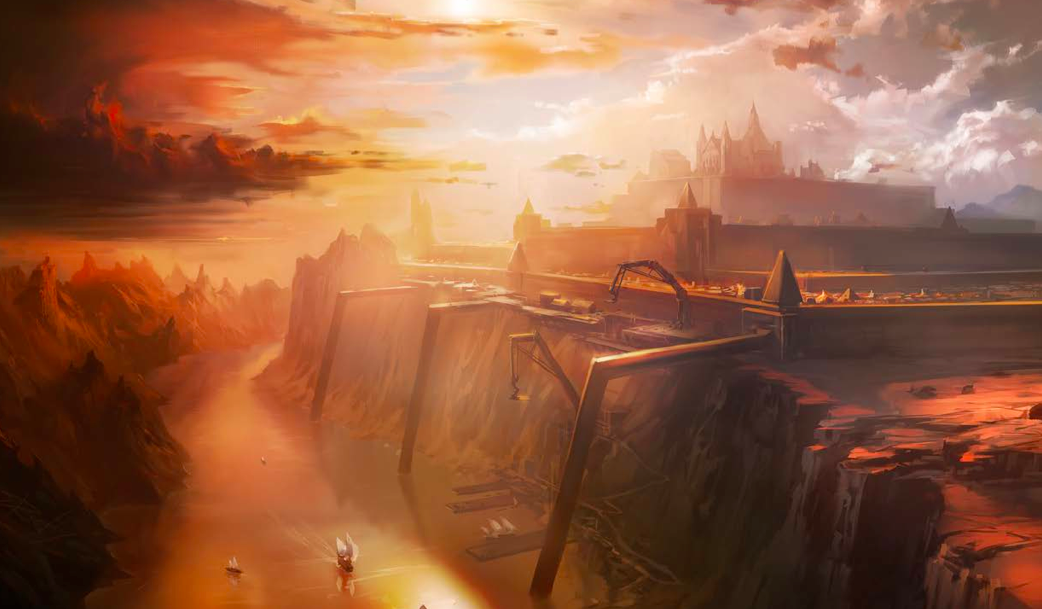
\includegraphics[width=12cm]{kenabres}

\bigskip
    
\vspace{7cm}

\begin{tabular} {cc}
\parbox{0.3\textwidth}{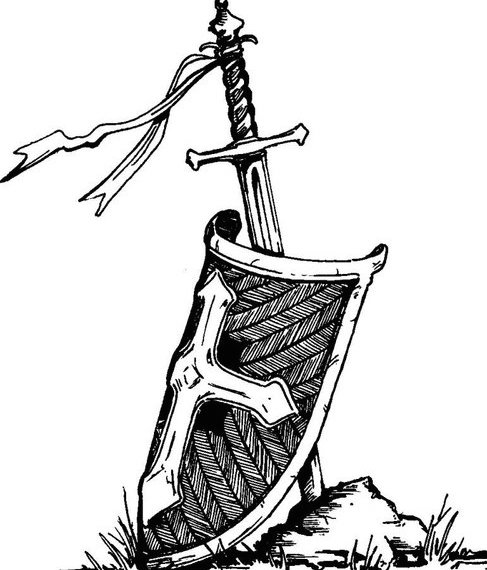
\includegraphics[width=2.5cm]{sword-shield}}
&
\parbox{0.7\textwidth}{{\Large\spacedlowsmallcaps{\mySubTitle}} \\ 

					{\normalsize
					
					\myGroup \\
					\myUrl \\
					\myTime}}
			\end{tabular}
\end{center}
\vfill
\end{titlepage}




%*******************************************************
% Colofone
%*******************************************************
\thispagestyle{empty}

\hfill

\vfill

\noindent\myName:
\textit{\myTitle,} \mySubTitle,
\textcopyright\ \the\year.

\medskip
\noindent{\spacedlowsmallcaps{Sito web}}: \\
\myUrl

\medskip
\noindent{\spacedlowsmallcaps{E-mail}}: \\
\mail{\myEmail}

\vspace{1cm}
\hrule
\bigskip

\noindent La pagina del titolo riporta l'immagine di copertina dell'avventura ``La piaga del mondo'' da cui il racconto \`e ispirato.
Alcuni dettagli fantastorici sono presi dal manuale ``Atlante del mare interno''.
Il logo spada e scudo in copertina \`e ripreso da angelfire7508 su Deviantart \url{http://angelfire7508.deviantart.com/art/Sword-and-Shield-original-47378670}.
\clearpage
%*******************************************************
% Abstract+Sommario
%*******************************************************

\selectlanguage{american}
\pdfbookmark{Abstract}{Abstract}
\begingroup
\let\clearpage\relax
\let\cleardoublepage\relax
\let\cleardoublepage\relax

\chapter*{Abstract}
In this story we talk about adventure. Set in Golarion and actually played in Pathfinder, the story unfolds in three chapters through which a group of adventurers will be bound to have a key role in the future of the troubled city of Kenabres.

\vfill

\selectlanguage{italian}
\pdfbookmark[1]{Sommario}{Sommario}
\chapter*{Sommario}
In questo racconto parliamo di avventura. Ambientata in Golarion e realmente giocata in Pathfinder, la storia si sviluppa in tre capitoli tramite i quali un gruppo di avventurieri sar\`a destinato ad avere un ruolo fondamentale per il futuro della travagliata citt\`a di Kenabres.

\endgroup			

\vfill


%%*******************************************************
% Ringraziamenti
%*******************************************************
\pdfbookmark{Ringraziamenti}{Ringraziamenti}

\begingroup
\let\clearpage\relax
\let\cleardoublepage\relax
\let\cleardoublepage\relax

\chapter*{Ringraziamenti}
Un sentito ringraziamento ai miei giocatori: Nicol\`o, Cristinan, Marco, Cecilia, Rita e Anna per aver contribuito agli aspetti pi\`u importanti della storia. Ringrazio gli amici per i consigli sulla stesura e i creatori di \LaTeX per la deliziosa qualit\`a del loro programma.
\endgroup




\clearpage
%************************************************
\chapter*{Antefatto}
\pdfbookmark[1]{Antefatto}{Antefatto}
%************************************************

Per decenni i demoni hanno invaso, saccheggiato e soggiogato la regione. Temibili creature di ogni tipo, con pelle dura come il ferro, denti affilati come lame e occhi brucianti come fiamme, hanno vagato per queste terre devastate che un tempo erano conosciute come il florido regno di Sarkoris. Quattro crociate sono state indette dai capi della chiesa di Iomedae e quelli di diverse altre religioni, con lo scopo di ripulire la macchia nota come ``Piaga del Mondo'': un flagello cosmico di dimensioni chilometriche delimitato da fiamme nere. Pi\`u ci si avvicina alla Piaga del Mondo, pi\`u il mondo fisico diventa imprevedibile. Il terreno cambia davanti ai propri occhi, mutando forma con contorta deliberazione che sembra terrorizzare la terra stessa. Laide creature vengono vomitate dalla follia al centro del flagello, mostruosit\`a provenienti dalle profondit\`a dell'Abisso hanno inflitto sconfitte sempre pi\`u miserabili alle armate dell'umanit\`a. Non fosse stato per le magiche Pietre Guardiane installate lungo i confini orientale e meridionale della regione, i demoni avrebbero da tempo invaso il settentrione del vicino regno di Mendev e forse ancora oltre. La Quarta Crociata \`e andata via via spegnendosi per alcuni, ma \`e molto viva per diversi altri. Quel che \`e certo \`e che le paralizzanti carenze di risultati hanno abbattuto il morale dei crociati, mettendo a serio rischio l'intera guerra. E sebbene l'inquietante influenza dei demoni cominci a penetrare la mente di troppi governanti, impegnati in un'intestina e quasi paranoica caccia alle streghe, una striminzita minoranza di prelati e paladini non solo sostiene che l'ultima battaglia sia ancora in corso, ma che nell'immediato futuro sar\`a evidente il suo esito. La Quarta Crociata non pu\`o essere definita vivace, ma i crociati ci hanno azzeccato pi\`u di quanto pensino circa l'arrivo imminente di una svolta. Una svolta destinata ad essere a favore dell'Abisso.
\clearpage
%*******************************************************
% Indice
%*******************************************************
\selectlanguage{italian}
\phantomsection
\pdfbookmark{\contentsname}{Indice}
\setcounter{tocdepth}{2}
\begingroup 
    \let\clearpage\relax
    \let\cleardoublepage\relax

    \tableofcontents
\endgroup
\markboth{\spacedlowsmallcaps{\contentsname}}{\spacedlowsmallcaps{\contentsname}} 

\begingroup 
    \let\clearpage\relax
    \let\cleardoublepage\relax
\endgroup

\pagestyle{scrheadings}
\cleardoublepage
%%******************************************************************
%% Mainmatter
%%******************************************************************
\pagenumbering{arabic}
%************************************************
\chapter{La caduta di Kenabres}
\label{chp:cap1}
%************************************************

La caduta. % La caduta di Kenabres
%************************************************
\chapter{Radianza, primo segnale di speranza}
\label{chp:cap2}
%************************************************

\`E l'anno 4692 quando Yaniel decide di annunciare pubblicamente il suo sdegno verso i crociati di Mendev. E non parliamo di una paladina qualsiasi, ma di un membro ufficiale dell'Ordine Brillante, nonch\'e conclamata cacciatrice di demoni. Yaniel, in un giorno di particolare ispirazione, decide infatti di manifestare ben pi\`u di un comune dissenso, rivolgendosi direttamente ai suoi commilitoni, accusandoli di negligenza e poltroneria. La dichiarazione avviene a gran voce con tanto di foglio di pergamena, nel bel mezzo della piazza di Clydwell e alla non casuale portata delle acute orecchie del prelato. Per la gente dell'epoca il riferimento di tali accuse \`e pi\`u che chiaro: \`e recentissima la ferita ancor pi\`u morale che fisica circa l'improvviso attacco di Khorramzadeh, meglio noto come il Signore delle Tempeste. Si narra infatti che poco prima che i difensori riuscissero a ricacciare lui e suoi famigli nell'Abisso, la Pietra Guardiana sia stata attaccata e persino scalfita da un fiammeggiante fendente dell'enorme demone. Sono dunque paura, incertezza e scoraggiamento i sentimenti che persistono sul morale dei cittadini di Kenabres, poich\'e stavolta neppure le poderose difese della loro citt\`a sono bastate a tenerli al sicuro.

Forse perch\`e le parole di Yaniel vanno troppo vicine alla realt\`a, la paladina viene presto sospesa dai suoi incarichi e infine scomunicata dal prelato. I suoi stessi superiori sono complici della severissima punizione. Disonorata e colta da mille emozioni, Yaniel reagisce di istinto, lasciando la citt\`a e decisa a riscattare se stessa tramite una santa e personale crociata. Assieme alla sua forza di volont\`a brandisce la sua clamorosa spada incantata, Radianza, conducendo la sua battaglia nel cuore del territorio dei demoni. Nei due anni successivi della paladina non si hanno pi\`u notizie e in Kenabres viene prontamente dichiarata dispersa.

\`E l'anno 4694 quando ella viene avvistata in prossimit\`a della Porta Nord. Barcollante ma fiera, porta Radianza saldamente in cinta e marcia a capo di un piccolo esercito di crociati liberati nel corso delle sue imprese. In quegli anni sia lei che i suoi ufficiali non sono pi\`u gli stessi. Da parte sua Yaniel ha rinunciato a un po' del suo orgoglio in favore dell'esperienza e delle difficili decisioni che un \emph{leader} \`e talvolta costretto ad affrontare; gli ufficiali e il prelato sono altres\`i pi\`u anziani, ma infine consapevoli che \`e proprio in momenti di crisi che la verit\`a \`e esattamente ci\`o che \`e necessario sentire.

Ahim\`e Yaniel viene assassinata prima della fine dell'anno, ad opera del lilitu Minagho, scovato dopo appena una settimana dall'inizio dell'ennesima spedizione. I seguaci di lei riescono fortunatamente a tornare in Kenabres, strappando Radianza dalle grinfie dell'Abisso ma perdendo traccia del corpo della prode guerriera, che purtroppo non viene pi\`u recuperato. La spada, come sensibile alla mancanza della sua eroina, cade in un'opaca oscurit\`a inibendo i suoi poteri. Nonostante ci\`o i crociati dichiarano la lama ``reliquia dell'Ordine Brillante'', esponendola in segno di rispetto nella prestigiosa vetrina della sede dell'Ordine: la Grigia Guarnigione.

A qualche mese dai nostri giorni Radianza viene saccheggiata da alcuni operatori occulti, probabilmente affiliati a una delle diverse organizzazioni criminali ormai radicate in citt\`a. Destino ha voluto che qualunque scellerato piano fosse riservato a Radianza non arrivasse mai a compimento, ma che piuttosto la mano di una nuova guerriera si stendesse sulla scintillante elsa dorata. Tra i sopravvisuti del disastro gira gi\`a voce che alcuni avventurieri stiano lottando tra le strade, liberando civili e annientando cultisti. Saranno forse loro a cambiare il corso della storia? % Radianza, primo segnale di speranza
%%************************************************
\chapter{La fine dello scoiattolo}
\label{chp:cap3}
%************************************************

Al quindicesimo giorno dall'incursione dei demoni in Kenabres, il gruppo di avventurieri si trova nel Librarium Alanera, esattamente nella zona opposta rispetto a casa Tirabade. Quella stessa notte un ricordo lontano prende posto nel sogno di Anvenn. Viaggiando indietro nel tempo, fino ai tempi della sua infanzia, egli si rivede tra le strade di Nisroch, una citt\`a portuale dell'ovest, in prossimit\`a della Baia del Conquistatore. Alcune scene, della durata di pochi minuti, vengono vissute da Avenn come fossero reali, ma accellerate. Le prime immagini sono piacevoli, i pensieri lo portano a rivivere alcuni momenti con i compagni di gilda. Ladri, fuorilegge e borseggiatori, ma anche filosofi, oratori e musicisti erano membri usuali della vecchia compagnia. Un attimo dopo risuonano rumori di passi, come in una marcia. Nella mente di Anvenn vengono visualizzati uomini in sandali, vestiti in tunica bianca e armati di pugni di ferro. Sono gli agenti di una societ\`a chiamata ``Sindone Silenziosa'', il giorno in cui il crudele governatore da inizio ad una folle caccia all'uomo.

Anvenn si risveglia di soprassalto, ma in mente ha uno specifico indirizzo e la criptica frase di addio di sua madre: ``sono una rosa mezza appassita''. In quell'epoca \`e una sacerdotessa di Desna, Veeruh, che gli salva la vita portandolo in Kenabres e affidandolo alla cura di una giovane e promettente iniziata: Irabeth Tirabade. \`E per motivi di sicurezza che Anvenn da quel giorno in avanti sar\`a conosicuto come Anevia, un nome che nel folclore Varisiano viene associato scaramanticamente alla carta della fortuna, lo \emph{scoiattolo}. La sua vita, dopotutto, non era stata da meno.

Anevia era l\`i il giorno dell'ultimo festival di Armasse, il giorno dell'attacco dei demoni. Caduta e poi gravemente ferita \`e grazie ad un colpo di fortuna se riesce a sopravvivere: un coraggioso gruppo di avventurieri la trova esanime in una buia caverna, indifesa ma viva. Un po' come anni prima Irabeth e Veeruh avevano fatto. Tuttavia presto o tardi gli interessi del gruppo si allontano dai suoi, la paura di non arrivare mai pi\`u a casa ha il sopravvento. Anevia, al quindicesimo giorno, decide di lasciare tutto e andare per la sua strada.

La sua scelta non \`e facile, n\'e gratuita. Ai membri pi\`u tenaci della compagnia, Gavin, Feanor e Seshilia \`e costretta a rivelare la sua identit\`a, ma \`e facendo leva sulla buon'anima di Amanil e Fratello Morrog che guadagna la  libert\`a di cercare il suo destino. Destino che si riveler\`a in fretta, come i suoi sogni: con passo lesto e qualche pozione di invisibilit\`a raggiunge casa, ma la scena che le si presenta \`e impietosa: muri gaffiati, silenzio assordante e puzzo di sangue accolgono il suo arrivo. \`E al suo primo passo oltre la soglia d'entrata che una voce grave e raschiante fa scattare la trappola: ``Sei dunque giunto, scoiattolino, il tuo cadavere sar\`a una dolce sorpresa per tua moglie''. Un mezzorco furfante di nome Vagrog, catturato anni prima da un arresto di Irabeth, ha scontato la sua pena ed \`e tornato dal suo esilio. Ci\`o nonostante la prigionia pare non abbia giovato al pericoloso criminale, che anzi \`e pronto a vendicarsi colpendo l'affetto pi\`u caro della sua arcinemica.

La storia di Anvenn o Anevia che dir si voglia finisce qui, stroncata da un magico tramortimento e un secondo prima che il suo cuore smetta di battere... 

Un piccolo \emph{crak} risuona all'istante dell'omicidio, una luce abbagliante irrompe dalle finestre e un calore avvolgente ma confortevole riempie la stanza. Una visione celestiale appare nella mente di tutte le donne e gli uomini nel raggio di diversi chilometri: una creatura umanoide vagamente attraente, adornata di corna di demonio e ali da pipistrello spunta evocata al cospetto di cinque condottieri in una sala circolare. La Pietra Guardiana non c'\`e pi\`u, distrutta in mille frammenti ha rilasciato una forma di energia cos\`i potente da richiamare Lady Vorlesh in persona, la fattucchiera delle recenti storie responsabile dell'invasione dei demoni nel nostro mondo. 

Come rinnovata da una forza dentro di lei, Anevia riprende conoscenza. Le sue mani sono bianche come la neve e i suoi capelli biondi come l'oro, due ali piumate le cingono la schiena e i fianchi. Le spoglie polverizzate di Vagrog le fanno compagnia sparse nel pavimento, nella strana ma autentica consapevolezza che lo stesso destino sia toccato a centinaia di agenti dell'Abisso cos\`i arroganti o sfortunati da trovarsi nel raggio di azione della Pietra. La fortuna dello scoiattolo forse \`e svanita, ma qualcosa di pi\`u grande ha riguadagnato il suo posto: la speranza.
 % Lo scoiattolo
%% *****************************************************************
%% Backmatter
%%******************************************************************
%\clearpage
%%*******************************************************
% Bibliografia
%*******************************************************
\nocite{*}
\printbibliography
\end{document}